\documentclass[11pt,reqno]{amsart}

\usepackage{amsthm,amsmath,amssymb}
\usepackage{mathtools}
\usepackage{proof}
\usepackage{xcolor}
\usepackage{graphicx,wrapfig}
\usepackage[T1]{fontenc}
\usepackage{courier}
\usepackage{hyperref}
\hypersetup{
    hidelinks=true
}
\usepackage{array}
\usepackage{multirow}
\usepackage{listings}
\lstset{basicstyle=\ttfamily\footnotesize, columns=fullflexible, language=C, morekeywords={omp,task,private,pragma,parallel,reduction,single,nowait,num_threads},frame=single, numbers=left}
\newcommand{\code}[1]{\texttt{#1}}
\newcommand\MyBox[2]{
  \fbox{\lower0.75cm
    \vbox to 1.7cm{\vfil
      \hbox to 1.7cm{\hfil\parbox{1.4cm}{#1\\#2}\hfil}
      \vfil}%
  }%
}
\graphicspath{ {./} }

\begin{document}

\begin{center}
\large\textbf{Assignment 1 - Part 1 \\ COMP529 Fall 2019 - Parallel Programming} \\
\normalsize\textbf{Erhan Tezcan 0070881 \\ 29.02.2020} \\
\end{center}

\section{Objective}

We are given a serial code implementation of John Conway's ``Game of Life''. This can be thought of as a stencil, where we work on a $2D$ array and for each cell we require information of the neighbor cells to do our computations. On each iteration, the result of a cell is written to the corresponding cell of another $2D$ array. Thus, we have 2 spatially identical arrays. We also plot one of the arrays on each iteration. In short, the two tasks we have can be denoted as:
\begin{itemize}
	\item \textbf{Compute} \\
	The cells are computed and results are written to the other array.
	\item \textbf{Plot} \\
	The resulting array is plotted. It is important to note that the array pointer given to the plotting function is of the array which we read from, so to see the results a swapping of pointers must occur right before the plotting.
\end{itemize}

We can also think of swapping as a task, but it is not task-parallelizable because swapping depends on the completion of both the plot and compute tasks, and consequently plot and compute tasks depend on the completion of swapping task. Furthermore, this is a very small task, literally three lines of code (one line if you remove newline characters!) that just swaps the pointers.
\begin{figure}[h]
\centering
\label{fig:ser}
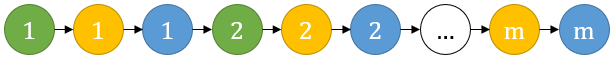
\includegraphics[width=0.75\linewidth]{serial_p1.png}
\caption{Serial Program. Green node is computation, yellow node is swapping, blue node is plotting. Numbers indicate the iteration. $m$ is the maximum number of iterations.}
\end{figure}

We can see on figure \ref{fig:ser} how the serial program runs. For each iteration, computation, swapping and plotting happens in order.

\section{Design and Implementation}

In my implementation, I have used \code{task} clause and nested parallelism. Before we begin to explain the details, we should explicitly state some constraints:
\begin{itemize}
	\item As stated in the previous section, swapping is not a parallelizable task.
	\item There needs to be a synchronization after plot and compute finishes right before swapping.
	\item Plot task always plots the already computed values.
	\item Plot task is not data-parallelizable. This is the case for both \code{gnuplot} and logging. We use logging to compare results, and to compare results we need to make sure about the order that the values are written. Therefore, we require serial plotting.
\end{itemize}

\begin{figure}[h]
\centering
\label{fig:par}
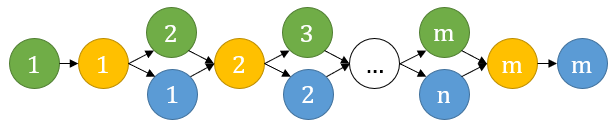
\includegraphics[width=0.75\linewidth]{parallel_p1.png}
\caption{Parallel Program. Green node is computation, yellow node is swapping, blue node is plotting. Numbers indicate the iteration. $m$ is the maximum number of iterations where $m=n+1$.}
\end{figure}

We can see on figure \ref{fig:par} how the parallel program runs. Now we will go into detail on how this works.
\subsection{Task Parallelism}
Here are the steps of task parallelism implemented in our code, as also seen on figure \ref{fig:par}.
\begin{enumerate}
	\item Compute and swap task runs in series, then the parallel region starts.
	\item A thread creates 2 tasks, where plotting task is taken by 1 thread, and it starts to plot the previous computation. Remaining $t-1$ threads are working on computation task.
	\item An implicit synchronization is achieved by closing the parallel region right before swapping. When the tasks finish, the program continues to swap and proceed to next iteration. These 2 steps happen for $m-1$ iterations.
	\item When the iteration loop finishes, we still have to plot the final computation, which happens outside the iteration loop.
\end{enumerate}

This way, we efficiently achieve task parallelism.

\subsection{Data Parallelism}
As we have noted before, we can't talk about data parallelism for swapping or plotting, however we can do it for the compute task. This task is all about doing computations on a matrix, therefore we can easily parallelize it using the \code{for} clause. The code is given on figure \ref{fig:dataparcompute}.

\begin{figure}[h]
\centering
\label{fig:dataparcompute}
\begin{lstlisting}
#pragma omp task
{
    #pragma omp parallel num_threads(numthreads-1) if(numthreads> 2)
    {
        #pragma omp for reduction(+: sum) private(j) 
        for(i=1;i<nx-1;i++) {
            for(j=1;j<ny-1;j++) {
                int nn = currWorld[i+1][j] + currWorld[i-1][j] + 
                    currWorld[i][j+1] + currWorld[i][j-1] + 
                    currWorld[i+1][j+1] + currWorld[i-1][j-1] + 
                    currWorld[i-1][j+1] + currWorld[i+1][j-1];
                nextWorld[i][j] = currWorld[i][j] ? 
                    (nn == 2 || nn == 3) : (nn == 3);
                sum += nextWorld[i][j];
            }
        } 
        #pragma omp single nowait
        {
            population[w_update] += sum;
        }
    }
}
\end{lstlisting}
\caption{Data Parallelized Computation Task}
\end{figure}

We see that we create many threads (excluding the one that was spent on plotting) and then use a basic \code{for} clause with reduction. This is also where we do a ``nested parallelism'', we were already in a \code{parallel} region when we launched these threads. We could parallelize both loops by using \code{collapse(2)} clause but the assignment asked for a $1D$ decomposition so we did not do that. To update the global sum after reductions we have a \code{single} clause, where \code{nowait} tells other threads to continue without waiting there if there is already a thread in there.

\subsection{Launch Parameters}

In addition to the given code, I have added a \code{-l} launch parameter that if given disables the logging function. Logging is writing the matrix to a file on each iteration, as if it is plotting it. This is done since it is not always possible to run \code{gnuplot} and furthermore we can compare the outputs of 2 programs using \code{diff} and comparing the outputs of two programs. If you do not pass \code{-l} option the program will take a lot of time!

\section{Experiments and Evaluation}
We have used \textbf{KUACC} for collecting performance data. The program was compiled with \code{GCC}. We conduct 2 experiments, where in one of them we fix the problem size while doubling the thread count (strong scaling) and on the other we fix the thread count to 16 and experiment with different problem sizes. We disable the plotting feature for these experiments, since plotting is a serial operation and it would create a critical path thus creating a lower bound for the shortest execution time which is at best as good as the serial time.  I have also used a single batch file for these experiments and also used the \code{--exclusive} option for the \code{sbatch} command to make sure it is only me that using the respective compute node.

\subsection{Experiment 1: Strong Scaling}
For the first experiment where we change the thread count, we provide two results: execution time and speedup.

\begin{figure}[h]
\centering
\label{fig:exp1_1}
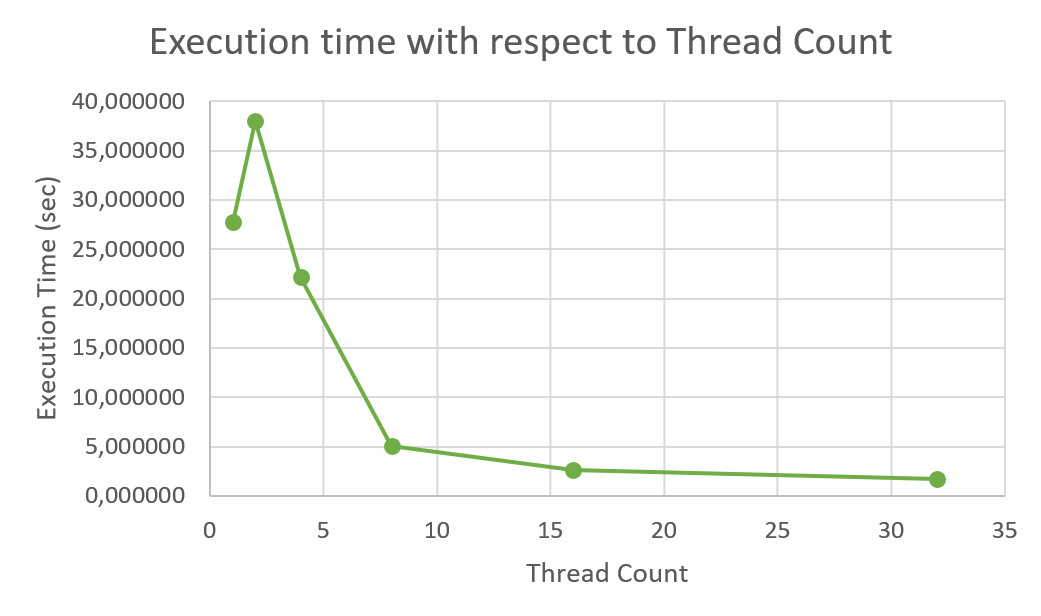
\includegraphics[width=0.8\linewidth]{exp1_1.png}
\caption{Execution Time versus Thread Count.}
\end{figure}

\begin{figure}[h]
\centering
\label{fig:exp1_2}
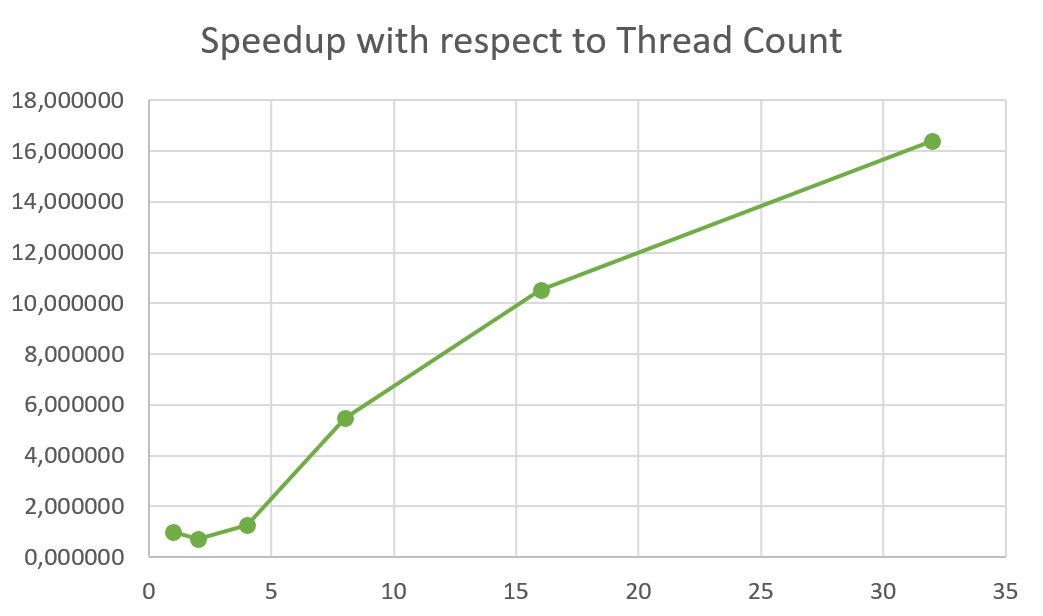
\includegraphics[width=0.8\linewidth]{exp1_2.png}
\caption{Speedup versus Thread Count.}
\end{figure}

From these graphs we can notice that having two threads versus one thread does not change much. In our code, when we have 1 thread executive the code without any \code{OpenMP} clauses or such, when we have multiple threads we use them. Given 2 threads, one of the threads go to the plotting task, the other one goes to the computing task. Considering the overhead of \code{OpenMP} instructions, we expect not much performance from the 2 thread implementation.  As we double our thread count, we expect to see halving of the execution time (thus doubling of the speedup) and it is evident that this is what we observe.

\subsection{Experiment 2: Adjusting Problem Size}
For the second experiment where we fix the thread count and increase the problem size, we again provide two results: execution time and approximate time spent per data point.

\begin{figure}[h]
\centering
\label{fig:exp2_1}
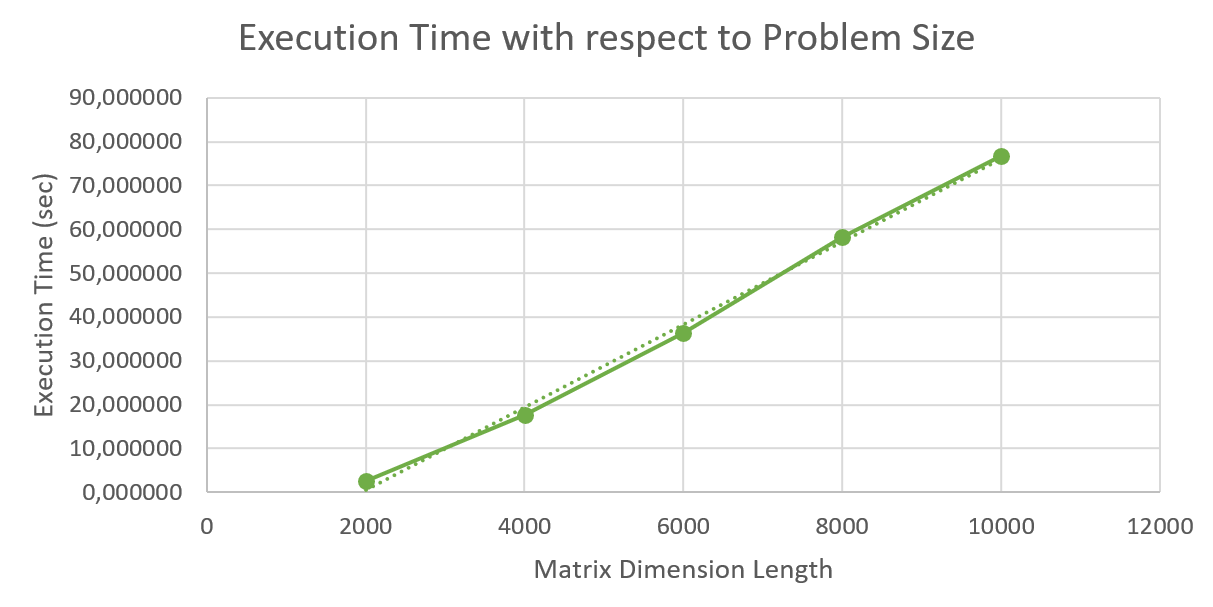
\includegraphics[width=0.8\linewidth]{exp2_1.png}
\caption{Execution time versus Problem Size.}
\end{figure}

\begin{figure}[h]
\centering
\label{fig:exp2_2}
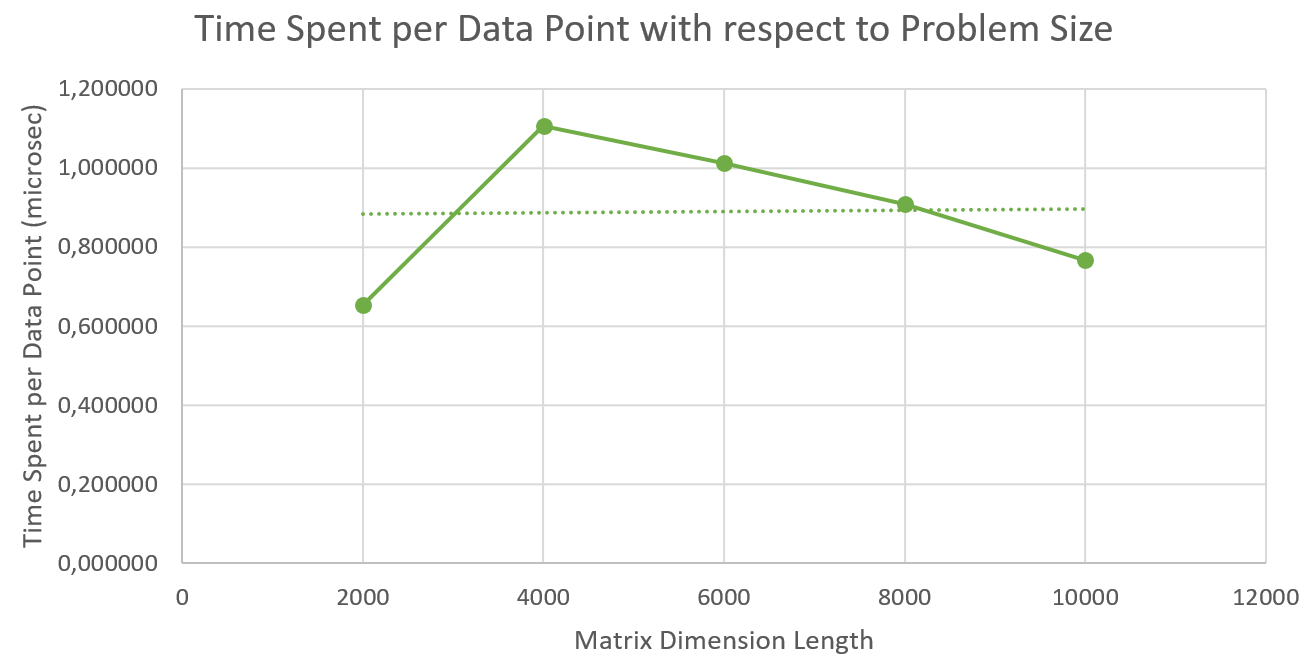
\includegraphics[width=0.8\linewidth]{exp2_2.png}
\caption{Approximate Time Spent per Data Point versus Problem Size.}
\end{figure}

On figure 6 we clearly see how the execution time increases linearly as the problem size gets bigger. We also added a regression line (shown dashed) that further indicates linear increase of the execution time. We have also added another plot where we calculate the approximate time spent on each data point. Ideally, we would expect this to stay at a constant value, and this is kind of what we observe as shown on figure 7. Though the results differ, the regression line is parallel to the problem size axis, which indicates on average the program spent same amount of time on each data point. 

\section{Conclusion}

We have achieved task and data parallelism. However, due to the nature of the plotting task, if we want to plot we do not gain any advantage of execution time. The actual data parallelism performance comes into play when we disable the plotting feature, and we have observed the expected linear correlation where doubling the thread count halved the execution time. Similarly, increasing problem size increased the execution time while the approximate time spent on each data point stayed closed to it's average value that was calculated over these experiments.
\end{document}